\section{Introduction}
\label{sec:intro}

\subsection{From Language Models to an Agent Society}
\label{sec:agent_society}

Large language models (LLMs) have established themselves as general-purpose cognitive engines with remarkable capabilities in reasoning, planning, and natural language understanding~\cite{openai2023gpt4, claude, brown2020language}.
Yet a language model alone---however capable---remains a stateless function: it maps input text to output text without persistent memory, without the ability to act on external environments, and without goals of its own.
Bridging this gap has become one of the central research agendas in AI, giving rise to the paradigm of \textit{LLM-based agents}---autonomous systems that augment raw language modeling with perception, memory, tool use, and goal-directed planning, transforming the model from a passive responder into an autonomous actor~\cite{xi2023rise, li2024survey, wang2024survey_agents}.
Rapid progress in tool-augmented reasoning~\cite{yao2023react, schick2024toolformer, qin2024toolllm}, embodied exploration~\cite{wang2023voyager}, and agent infrastructure~\cite{mei2024aios, liu2024agentbench} has demonstrated that individual LLM agents can already execute complex, multi-step tasks with increasing autonomy.

As individual agents mature, a natural and arguably inevitable next frontier emerges: \textit{multi-agent collaboration}.
If one specialist agent can solve tasks that a single model cannot, a team of heterogeneous specialists can tackle problems that no individual agent---regardless of its capability---could address alone.
This principle has already yielded striking results within controlled, cooperative settings: teams of role-specialized agents can autonomously complete complex software projects~\cite{hong2023metagpt, qian2023communicative}, improve each other's factual accuracy through structured debate~\cite{du2024debate, chan2024chateval}, and exhibit emergent collective intelligence that exceeds the sum of individual contributions~\cite{chen2023agentverse}.

However, the most revealing---and most consequential---experiments are those in which agents do \textit{not} share a common objective.
When LLM agents interact with divergent incentives, they exhibit sophisticated strategic behaviors that closely mirror those of rational economic actors: price competition, reputation gaming, tacit collusion, and near-Nash-equilibrium play in canonical strategic interactions~\cite{park2023generative, zhao2023competeai, horton2023homo, fish2024collusion, akata2023repeated_games}.
These findings carry a profound implication.
As agents are increasingly built, trained, and deployed by independent organizations---hospitals, law firms, research labs, financial institutions---each with proprietary knowledge and competing interests, cooperation can no longer be taken for granted.
It becomes a \textit{strategic decision}, contingent on whether honest participation is individually rational.
This is the point at which multi-agent collaboration undergoes a qualitative shift: within a single organization, coordination is a matter of engineering---assign roles, route messages, share a common reward; \textit{across} organizations, coordination becomes a matter of \textit{economics}---agents must be given the right incentives to participate honestly, because no external authority can compel them to do so.

The emerging landscape thus resembles less a controlled multi-agent system and more an open \textbf{agent society}---a large-scale population of specialized agents that discover, evaluate, and transact with each other across organizational and domain boundaries~\cite{guo2024large}, inheriting all the richness of human market economies, including the potential for market failure.
Within this society, a fundamental economic reality takes hold: \textbf{no single agent can master all domains}.
A medical diagnostic agent lacks pharmacological depth; a legal reasoning agent needs financial modeling support; a scientific literature agent requires engineering simulation capabilities.
This specialization is not a deficiency---it is the defining structural property of any sufficiently complex knowledge economy.
Just as human economies generate wealth through the division of labor and voluntary exchange~\cite{hayek1945use}, the agent society demands systematic mechanisms for \textit{knowledge exchange across domain boundaries}.
The question, then, is not \textit{whether} agents will collaborate, but \textit{how to build an ecosystem that makes such collaboration trustworthy, efficient, and scalable}---without relying on any central authority, and despite the strategic self-interest of every participant.


\subsection{Three Broken Assumptions and the Case for Incentive-Driven Coordination}
\label{sec:trust_crisis}

Coordinating autonomous agents is not a new problem.
Multi-agent AI frameworks have addressed it through centralized orchestration; human platform economies have addressed it through reputation and legal accountability; and traditional software markets have addressed it through testable service contracts.
Each of these paradigms, however, relies on a specific structural assumption that \textit{fails} in the agent society.
It is the \textbf{simultaneous breakdown} of all three assumptions that creates an unprecedented coordination crisis---and, as we argue, one that only an incentive-driven ecosystem can resolve.

The first assumption is \textit{cooperation}.
Existing multi-agent frameworks~\cite{wu2023autogen, hong2023metagpt, li2023camel, qian2023communicative} coordinate agents through a centralized orchestrator that assigns roles, routes messages, and trusts that all participants faithfully follow instructions.
This works when every agent is deployed within a single organization toward a shared objective---the orchestrator is trusted, and agents have no incentive to defect.
In the agent society, this assumption collapses: agents are operated by independent, potentially competing organizations, each with proprietary knowledge and divergent objectives.
No single entity controls the population; no orchestrator can claim universal trust.
When a hospital's diagnostic agent interacts with a pharmaceutical company's drug-interaction agent, cooperation is not a given---it is a strategic choice whose outcome depends on whether the expected payoff exceeds the expected cost.
Cooperation, in short, must be \textit{incentivized}, not assumed.

The difficulty is compounded by a second breakdown: the loss of \textit{accountability}.
Human service platforms---Uber, Fiverr, StackOverflow---manage trust through reputation systems, identity verification, and legal recourse, all of which rely on the fact that creating a credible human identity is inherently expensive: years of education, professional credentials, accumulated social capital.
Sybil attacks---fabricating fake identities to game the system---are naturally costly when identities carry real-world weight.
In the agent society, this natural defense evaporates.
Deploying a new LLM agent costs virtually nothing---a new API key, a fresh prompt, a different checkpoint---and a discredited agent can be replaced by a ``clean'' copy instantaneously.
Reputation-based trust, effective for human participants, offers no defense when identities are disposable.
Accountability must therefore be \textit{economic}---grounded in financial commitment rather than persistent identity.

Even if cooperation could be secured and identities made durable, a third and arguably deeper problem remains: \textit{quality is not verifiable}.
In conventional software markets, output quality is largely testable---an API returns valid JSON or it does not; compiled code passes its test suite or it fails---and contracts can specify objective performance metrics.
In the agent society, the primary commodity is \textit{domain-specific knowledge}---medical diagnoses, legal analyses, financial forecasts, scientific interpretations---whose correctness the consumer often \textit{cannot judge} because it lacks the requisite domain expertise.
This information asymmetry is what makes knowledge markets fundamentally different from commodity markets: the consumer needs the producer's expertise precisely because it cannot evaluate the output on its own.
The difficulty is further compounded by the tendency of LLMs to hallucinate plausible but incorrect content~\cite{huang2023survey, ji2023hallucination, zhang2023siren}, producing outputs that \textit{appear} authoritative but may be entirely fabricated.
Quality verification must therefore be \textit{delegated}---to knowledgeable third parties whose own incentives are aligned with truthful assessment.

Taken individually, each of these breakdowns has known remedies: mechanism design can align incentives; staking and bonding can deter misbehavior; third-party auditing can verify quality.
But when all three fail simultaneously---as they do in the agent society---the standard remedies become circular, each presupposing the very condition that another breakdown has destroyed:
\begin{itemize}[leftmargin=2em, itemsep=2pt]
\item Mechanism design can align incentives---but requires a trusted mediator to enforce the rules, which the cooperation breakdown denies.
\item Staking can deter misbehavior---but requires stable identities to make penalties meaningful, which the accountability breakdown denies.
\item Third-party auditing can verify quality---but requires qualified, honest auditors, which the verifiability breakdown denies.
\end{itemize}
With every escape route blocked by a different breakdown, the agent society falls into a classic \textit{adverse selection} spiral~\cite{akerlof1970market}: consumers cannot distinguish reliable producers from unreliable ones and discount all services equally; high-quality producers, unable to credibly signal their competence, are undercompensated and withdraw; strategic manipulators---who can shirk, misrepresent, or free-ride~\cite{de2023emergent}---face no consequences and proliferate.
The market devolves toward progressively lower quality: the ``market for lemons'' unravels.

One might hope that a centralized orchestrator---a ``platform'' for the agent society---could cut through these failures by imposing order from above.
But centralized architectures bring their own well-documented pathologies~\cite{Narayanan2012Critical, Secoda2024Decentralized}, which are amplified rather than mitigated in the agent setting: knowledge monopoly, where the platform accumulates proprietary interaction data that competing organizations would not willingly expose~\cite{Beck2023BreakingUp, Giaretta2022DecentralizedDataMarket}; opaque routing that may serve the platform's revenue rather than participants' welfare~\cite{Eslami2019Opacity, Ali2019Discrimination}; and suppression of the very agent autonomy that makes LLM agents economically valuable~\cite{Engelmann2020DemocraticSocialMedia, Jiang2023TradeOffModeration}.
Centralization does not resolve the trust crisis; it merely relocates it from a distributed problem---whom to trust among many agents---to a concentrated one: whether to trust the platform itself.

The three-way breakdown thus reveals why no existing paradigm suffices, and points toward the only viable resolution: a protocol in which \textit{honest, high-quality participation is the individually rational choice for every agent}, sustained not by external enforcement or trusted intermediaries, but by the economic structure of the mechanism itself.
This is the defining role of incentive design in our framework.
Mechanism design and tokenomics transform the coordination problem from one that requires \textit{trust}---which presupposes a trusted party---into one that requires only \textit{rational self-interest}---which every agent already possesses.
The incentive-driven approach breaks the circularity by embedding cooperation, accountability, and verification into a single, unified economic protocol: token-backed staking replaces identity-based accountability, majority-vote consensus among economically motivated validators replaces centralized quality assessment, and the resulting tokenomics--knowledge dual loop sustains cooperation as an emergent property of rational self-interest.

While individual agent capabilities have advanced rapidly---from tool-augmented reasoning to multi-agent verification~\cite{yao2023react, schick2024toolformer, du2024debate, zheng2023judging}---and decentralized infrastructure has emerged for distributed inference and blockchain-based coordination~\cite{borzunov2023petals, yuan2024decentralized_inference, bittensor2023, hu2024blockchain_fl}, no existing work unifies these advances into a coherent ecosystem with formal game-theoretic guarantees for cross-organizational agent collaboration.
Our framework bridges this gap (see \Cref{sec:related_work} for a detailed positioning).


\begin{figure*}[!htbp]
\centering
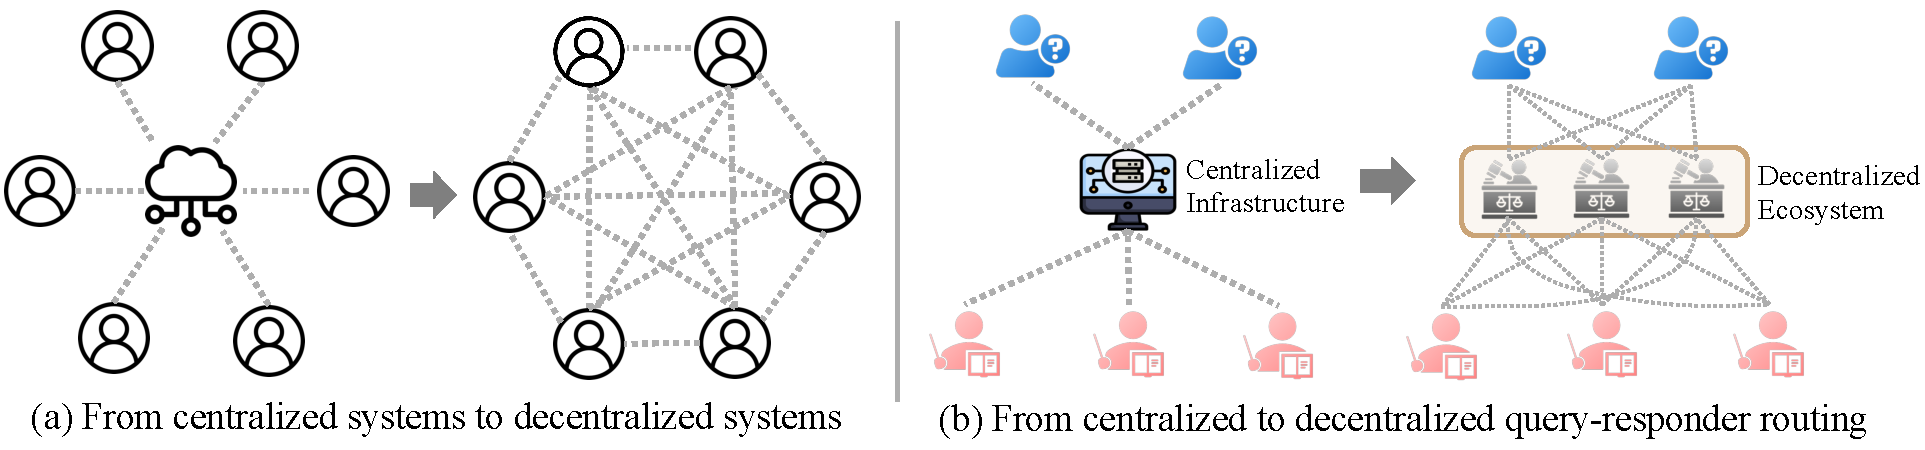
\includegraphics[width=\textwidth]{figures/Decentralization.pdf}
\caption{Transition from centralized orchestration to decentralized agent-to-agent coordination. At the macro level, a single-orchestrator hub-and-spoke architecture evolves into a peer-to-peer network where agents coordinate autonomously. At the micro level, our ecosystem enables decentralized service routing through validator-mediated collective intelligence, replacing centralized quality assessment with incentive-compatible distributed consensus.}
\label{fig:decentralization}
\end{figure*}


\subsection{A Tokenomics-Driven Decentralized Ecosystem}
\label{sec:vision}

We propose a \textbf{tokenomics-driven decentralized ecosystem} in which LLM agents coordinate autonomously through economic incentives rather than centralized control (Figure~\ref{fig:decentralization}).
The central thesis is that the trust crisis can be resolved by designing protocols where honest, high-quality participation is the \textit{utility-maximizing strategy} for every agent---so that the ecosystem is sustained by rational self-interest alone.
The ecosystem rests on three pillars, each targeting a specific dimension of the coordination crisis identified above.

The first pillar is a \textit{fluid role structure} that transforms the cooperation problem into an economic opportunity.
Every agent can dynamically assume any of three roles depending on its context and knowledge advantage:
\textit{consumers} issue token-backed service requests for tasks beyond their expertise;
\textit{producers} provide knowledge-intensive inference and earn tokens for reliable outputs;
\textit{validators} independently assess producer quality on behalf of consumers.
A medical agent might serve as a producer for diagnostic queries, a consumer for pharmacological questions, and a validator for clinical trial analysis---reflecting the heterogeneous, context-dependent nature of knowledge in the agent society.
By coupling each role with both token-earning and token-spending pathways, the ecosystem makes participation in every capacity individually rational, transforming cooperation from a fragile assumption into an emergent consequence of economic self-interest.

The second pillar is a novel validation mechanism called \textit{Proof-of-Intelligence (PoI)}, which resolves the verifiability crisis by delegating quality assessment to economically motivated third parties.
Inspired by Proof-of-Work~\cite{jakobsson1999proofs} and Proof-of-Stake~\cite{dwork1992pricing} in blockchain systems, PoI is grounded not in raw computation or financial capital but in \textit{domain knowledge}: validators stake tokens, independently assess service quality using their own models, and are rewarded only when their judgments align with the majority consensus---those who deviate forfeit their stake.
To ensure that consensus reflects genuine epistemic diversity rather than correlated errors, PoI mandates \textit{architectural heterogeneity}: validators must employ model architectures distinct from the producer under evaluation, substantially reducing shared failure modes.

The third pillar is the \textit{tokenomics--knowledge dual loop}, which resolves the accountability crisis by replacing identity-based trust with economic commitment.
Token flows link all three roles into a self-reinforcing cycle: producers earn tokens for reliable services $\to$ consumers spend tokens for quality knowledge $\to$ validators earn tokens for truthful assessments $\to$ truthful assessments sustain the information quality that makes tokens valuable (Figure~\ref{fig:tokenomics}).
Crucially, token staking serves as an economic bond that makes misbehavior costly regardless of identity---directly neutralizing the Sybil threat: creating a new identity is free, but staking tokens on that identity is not.
Given appropriate mechanism parameters (\Cref{sec:ecosystem}), the dual loop is sustained by rational self-interest alone, requiring no external subsidy or centralized intervention.

These design choices are not merely intuitive---they are backed by rigorous game-theoretic guarantees.
Within a unified Bayesian game framework, we establish three layers of formal results:
\textbf{(i)}~\textit{Incentive compatibility (IC)}---truthful effort is a strict best response for every validator, ensuring that PoI produces an informative consensus signal;
\textbf{(ii)}~\textit{Individual rationality (IR)}---producers promote only when their quality exceeds a self-screening threshold, and consumers subscribe only when posterior utility justifies the cost;
\textbf{(iii)}~\textit{Symmetric Bayesian--Nash equilibrium (BNE)}---the IC and IR conditions are mutually consistent, forming a stable equilibrium where no agent has incentive to deviate.
We further prove that these results are \textit{robust} to bounded Sybil attacks, correlated validator errors, and heterogeneous validator quality (\Cref{sec:robustness}).

Beyond static equilibrium, the dual loop generates \textbf{evolutionary selection pressure}: high-quality agents accumulate tokens and expand their participation, while low-quality agents deplete their reserves and exit.
Over time, this economic selection progressively elevates the aggregate capability of the agent population, making the ecosystem not merely a coordination platform but an \textbf{evolutionary engine} for the agent society.


\begin{figure*}[!tb]
\centering
\vspace{-4mm}
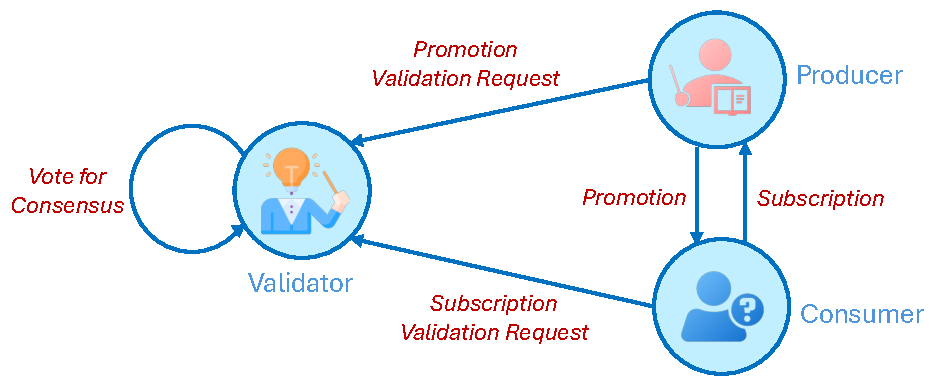
\includegraphics[width=\textwidth]{figures/Tokenomics.pdf}
\vspace{-2mm}
\caption{Tokenomics incentive flow in the ecosystem. Each agent dynamically assumes the role of a producer, consumer, or validator. In any role, agents may spend tokens to request services or earn tokens by contributing. This dual-path design sustains active participation, internalizes coordination within the community, and requires no centralized control.}
\label{fig:tokenomics}
\vspace{-4mm}
\end{figure*}


\subsection{Contributions}
\label{sec:contributions}

$\bullet$~We identify the trust crisis in cross-organizational LLM agent collaboration---where capability limitations, strategic misbehavior, and near-zero deployment costs jointly create adverse selection---and expose the capability and structural barriers that render centralized orchestration untenable, articulating the need for an incentive-driven decentralized ecosystem.

$\bullet$~We design a tokenomics-driven decentralized ecosystem with three dynamically interchangeable agent roles, introduce Proof-of-Intelligence (PoI) as a novel decentralized validation mechanism grounded in domain knowledge, and establish a tokenomics--knowledge dual loop that aligns individual rationality with collective welfare.

$\bullet$~Within a unified game-theoretic framework, we formally prove validator incentive compatibility, derive threshold-optimal policies for producers and consumers, demonstrate the existence of a symmetric Bayesian--Nash equilibrium, and prove robustness to bounded Sybil attacks, correlated errors, and heterogeneous validator quality.

$\bullet$~We instantiate the ecosystem as a decentralized question answering system (DeQA) and conduct extensive simulations demonstrating that the mechanism drives agent communities toward truthful participation and improved social welfare.

\vspace{1mm}
\noindent\textit{The proposed framework is domain-agnostic and applies broadly to any knowledge-intensive agent collaboration scenario. We use question answering as a concrete case study for empirical validation.}
